% answers.tex —— 1987 年·全国卷·文科 · 参考答案与详细解析片段
% 由 tools/generate_projects.py 依来源总账自 1987/1987_数学真题_全国文_试题.md + 1987/1987_数学真题_全国文_解析正文.md + 1987/1987_数学真题_全国文_答案要点.md 生成，勿手改（改源 MD 后重跑）


\begin{gktip}
固定源 PDF 只有一页原卷题面，原卷页码为 31，不含答案和解析页。下列推导均为本库独立复算。第 22 题的条件实际允许两个正方形面积，不能据“求面积”四字擅自挑选一个。
\end{gktip}

\begin{answer}
\gksolhead{1}{}

\textbf{题目}：

设 $S,T$ 是两个非空集合，且 $S\nsubseteq T,\ T\nsubseteq S$，令 $X=S\cap T$，那么 $S\cup X$ 等于\mbox{（　　）}

（A）$X$　　（B）$T$　　（C）$\varnothing$　　（D）$S$

\Needspace{4\baselineskip}
\textbf{解析}

\Needspace{5\baselineskip}
集合吸收律给出

\nopagebreak[4]
\[
S\cup X=S\cup(S\cap T)=S.
\]

\gkanswer{答案：D}

\end{answer}
\begin{answer}
\gksolhead{2}{}

\textbf{题目}：

\Needspace{5\baselineskip}
设椭圆方程为

\nopagebreak[4]
\[
\frac{x^2}{a^2}+\frac{y^2}{b^2}=1\qquad(a>b>0),
\]

令 $c=\sqrt{a^2-b^2}$，那么它的准线方程为\mbox{（　　）}

（A）$y=\pm\dfrac{a^2}{c}$　　（B）$y=\pm\dfrac{b^2}{c}$

（C）$x=\pm\dfrac{a^2}{c}$　　（D）$x=\pm\dfrac{b^2}{c}$

\Needspace{4\baselineskip}
\textbf{解析}

\Needspace{5\baselineskip}
椭圆的离心率为 $e=c/a$，长轴在 $x$ 轴上，准线为

\nopagebreak[4]
\[
x=\pm\frac ae=\pm\frac{a^2}{c}.
\]

\gkanswer{答案：C}

\end{answer}
\begin{answer}
\gksolhead{3}{}

\textbf{题目}：

设 $\log_3 4\cdot\log_4 8\cdot\log_8m=\log_4 16$，那么 $m$ 等于\mbox{（　　）}

（A）$\dfrac92$　　（B）$9$　　（C）$18$　　（D）$27$

\Needspace{4\baselineskip}
\textbf{解析}

\Needspace{5\baselineskip}
利用换底公式

\nopagebreak[4]
\[
\log_3 4\cdot\log_4 8\cdot\log_8m
=\log_3m.
\]

右端 $\log_4 16=2$，故 $\log_3m=2$，得到 $m=9$。

\gkanswer{答案：B}

\end{answer}
\begin{answer}
\gksolhead{4}{}

\textbf{题目}：

复数 $\sin40^\circ-i\cos40^\circ$ 的辐角为\mbox{（　　）}

（A）$40^\circ$　　（B）$140^\circ$　　（C）$220^\circ$　　（D）$310^\circ$

\Needspace{4\baselineskip}
\textbf{解析}

\nopagebreak[4]
\[
\sin40^\circ-i\cos40^\circ
=\cos50^\circ-i\sin50^\circ
=\cos310^\circ+i\sin310^\circ.
\]

所以其辐角为 $310^\circ$。

\gkanswer{答案：D}

\end{answer}
\begin{answer}
\gksolhead{5}{}

\textbf{题目}：

二次函数 $y=f(x)$ 的图象如图所示，那么此函数为\mbox{（　　）}
\nopagebreak[4]
\begin{center}% 1987 年全国卷文科第 5 题：二次函数图象
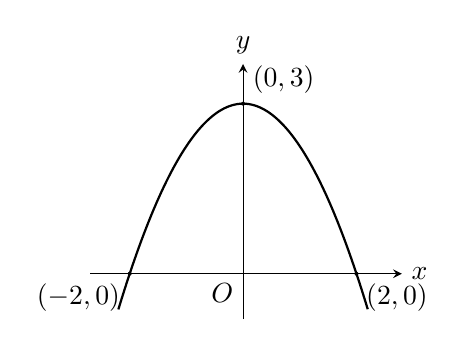
\begin{tikzpicture}[scale=0.72,>=stealth]
  \draw[->] (-2.7,0)--(2.8,0) node[right] {$x$};
  \draw[->] (0,-0.8)--(0,3.7) node[above] {$y$};
  \draw[thick,domain=-2.2:2.2,samples=100]
    plot (\x,{3-0.75*\x*\x});
  \fill (-2,0) circle (1pt) node[below left] {$(-2,0)$};
  \fill (2,0) circle (1pt) node[below right] {$(2,0)$};
  \fill (0,3) circle (1pt) node[above right] {$(0,3)$};
  \node[below left] at (0,0) {$O$};
\end{tikzpicture}
\end{center}
\nopagebreak[4]
（A）$y=x^2-4$　　（B）$y=4-x^2$

（C）$y=\dfrac34(4-x^2)$　　（D）$y=\dfrac34(2-x^2)$

\Needspace{4\baselineskip}
\textbf{解析}

\Needspace{5\baselineskip}
图象的顶点为 $(0,3)$，与 $x$ 轴交于 $(-2,0)$、$(2,0)$，故

\nopagebreak[4]
\[
y=c(4-x^2),\qquad 4c=3.
\]

\Needspace{5\baselineskip}
所以函数为

\nopagebreak[4]
\[
y=\frac34(4-x^2).
\]

\gkanswer{答案：C}

\end{answer}
\begin{answer}
\gksolhead{6}{}

\textbf{题目}：

在区间 $(-\infty,0)$ 上为增函数的是\mbox{（　　）}

（A）$y=-\log_{\frac12}(-x)$　　（B）$y=\dfrac{x}{1-x}$

（C）$y=-(x+1)^2$　　（D）$y=1+x^2$

\Needspace{4\baselineskip}
\textbf{解析}

\Needspace{5\baselineskip}
选项（B）中

\nopagebreak[4]
\[
\left(\frac{x}{1-x}\right)'=\frac1{(1-x)^2}>0,
\]

所以它在 $(-\infty,0)$ 上递增。其余选项不满足全区间的递增性。

\gkanswer{答案：B}

\end{answer}
\begin{answer}
\gksolhead{7}{}

\textbf{题目}：

已知平面上一点 $P$ 在原坐标系中的坐标为 $(0,m)$（$m\ne0$），而在平移后所得到的新坐标系中的坐标为 $(m,0)$，那么新坐标系的原点 $O'$ 在原坐标系中的坐标为\mbox{（　　）}

（A）$(-m,m)$　　（B）$(m,-m)$　　（C）$(m,m)$　　（D）$(-m,-m)$

\Needspace{4\baselineskip}
\textbf{解析}

\Needspace{5\baselineskip}
设新原点在原坐标系中的坐标为 $(u,v)$。平移后点 $P$ 的坐标满足

\nopagebreak[4]
\[
(0-u,m-v)=(m,0).
\]

故 $u=-m,\ v=m$，新原点为 $(-m,m)$。

\gkanswer{答案：A}

\end{answer}
\begin{answer}
\gksolhead{8}{}

\textbf{题目}：

\Needspace{5\baselineskip}
要得到函数

\nopagebreak[4]
\[
y=\sin\left(2x-\frac\pi3\right)
\]

的图象，只需将函数 $y=\sin2x$ 的图象（如图）\mbox{（　　）}
\nopagebreak[4]
\begin{center}% 1987 年全国卷文科第 8 题：y=sin 2x 图象
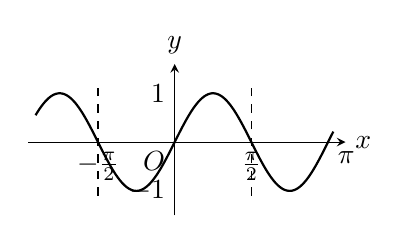
\begin{tikzpicture}[scale=0.62,>=stealth]
  \draw[->] (-3.0,0)--(3.5,0) node[right] {$x$};
  \draw[->] (0,-1.5)--(0,1.6) node[above] {$y$};
  \draw[thick,domain=-2.85:3.25,samples=160]
    plot (\x,{sin(114.592*\x)});
  \draw[dashed] (-1.57,-1.1)--(-1.57,1.1);
  \draw[dashed] (1.57,-1.1)--(1.57,1.1);
  \node[below] at (-1.57,0) {$-\frac\pi2$};
  \node[below] at (1.57,0) {$\frac\pi2$};
  \node[below right] at (3.14,0) {$\pi$};
  \node[left] at (0,1) {$1$};
  \node[left] at (0,-1) {$-1$};
  \node[below left] at (0,0) {$O$};
\end{tikzpicture}
\end{center}
\nopagebreak[4]
（A）向左平行移动 $\dfrac\pi3$　　（B）向右平行移动 $\dfrac\pi3$

（C）向左平行移动 $\dfrac\pi6$　　（D）向右平行移动 $\dfrac\pi6$

\Needspace{4\baselineskip}
\textbf{解析}

\nopagebreak[4]
\[
\sin\left(2x-\frac\pi3\right)
=\sin\left(2\left(x-\frac\pi6\right)\right).
\]

所以将 $y=\sin2x$ 的图象向右平移 $\frac\pi6$。

\gkanswer{答案：D}

\end{answer}
\begin{answer}
\gksolhead{9}{}

\textbf{题目}：

求函数 $y=\sin^2 2x$ 的周期。

\Needspace{4\baselineskip}
\textbf{解析}

\nopagebreak[4]
\[
\sin^22x=\frac{1-\cos4x}{2}.
\]

\Needspace{5\baselineskip}
因此最小正周期为

\nopagebreak[4]
\[
\frac{2\pi}{4}=\frac\pi2.
\]

\gkanswer{答案：$\dfrac\pi2$}

\end{answer}
\begin{answer}
\gksolhead{10}{}

\textbf{题目}：

\Needspace{5\baselineskip}
已知方程

\nopagebreak[4]
\[
\frac{x^2}{2+\lambda}-\frac{y^2}{1+\lambda}=1
\]

表示双曲线，求 $\lambda$ 的范围。

\Needspace{4\baselineskip}
\textbf{解析}

\Needspace{5\baselineskip}
要使

\nopagebreak[4]
\[
\frac{x^2}{2+\lambda}-\frac{y^2}{1+\lambda}=1
\]

\Needspace{5\baselineskip}
表示双曲线，两个分母必须同号且不为零：

\nopagebreak[4]
\[
(\lambda+2)(\lambda+1)>0.
\]

\Needspace{5\baselineskip}
所以

\nopagebreak[4]
\[
\lambda\in(-\infty,-2)\cup(-1,+\infty).
\]

\gkanswer{答案：$\lambda\in(-\infty,-2)\cup(-1,+\infty)$}

\end{answer}
\begin{answer}
\gksolhead{11}{}

\textbf{题目}：

若 $(1+x)^n$ 的展开式中，$x^3$ 的系数等于 $x$ 的系数的 7 倍，求 $n$。

\Needspace{4\baselineskip}
\textbf{解析}

\Needspace{5\baselineskip}
由二项式系数

\nopagebreak[4]
\[
\binom n3=7\binom n1=7n,
\]

\Needspace{5\baselineskip}
得

\nopagebreak[4]
\[
(n-1)(n-2)=42.
\]

取正整数解 $n=8$。

\gkanswer{答案：$n=8$}

\end{answer}
\begin{answer}
\gksolhead{12}{}

\textbf{题目}：

\Needspace{5\baselineskip}
求极限

\nopagebreak[4]
\[
\lim_{n\to\infty}\left(
\frac1{n^2}+\frac2{n^2}+\frac3{n^2}
+\cdots+\frac{2n}{n^2}\right).
\]

\Needspace{4\baselineskip}
\textbf{解析}

\Needspace{5\baselineskip}
前 $2n$ 个正整数的和为 $n(2n+1)$，故

\nopagebreak[4]
\[
\lim_{n\to\infty}
\frac{1+2+\cdots+2n}{n^2}
=\lim_{n\to\infty}\frac{n(2n+1)}{n^2}=2.
\]

\gkanswer{答案：$2$}

\end{answer}
\begin{answer}
\gksolhead{13}{}

\textbf{题目}：

由数字 $1,2,3,4,5$ 组成没有重复数字且数字 1 与 2 不相邻的五位数。求这种五位数的个数。

\Needspace{4\baselineskip}
\textbf{解析}

五个数字全排列有 $5!=120$ 种。1、2 相邻时作为一个整体，内部有 2 种顺序，与其他三个数字共作 $4!$ 排列，故有 $2\cdot4!=48$ 种。

\Needspace{5\baselineskip}
所求个数为

\nopagebreak[4]
\[
5!-2\cdot4!=72.
\]

\gkanswer{答案：$72$}

\end{answer}
\begin{answer}
\gksolhead{14}{}

\textbf{题目}：

\Needspace{5\baselineskip}
求函数

\nopagebreak[4]
\[
y=\log_2(1+2x-3x^2)
\]

的定义域。

\Needspace{4\baselineskip}
\textbf{解析}

\Needspace{5\baselineskip}
对数真数必须为正：

\nopagebreak[4]
\[
1+2x-3x^2=(1-x)(3x+1)>0.
\]

\Needspace{5\baselineskip}
所以定义域为

\nopagebreak[4]
\[
\left(-\frac13,1\right).
\]

\gkanswer{答案：$\left(-\dfrac13,1\right)$}

\end{answer}
\begin{answer}
\gksolhead{15}{}

\textbf{题目}：

圆锥底面积为 $3\pi$，母线与底面所成的角为 $60^\circ$，求它的体积。

\Needspace{4\baselineskip}
\textbf{解析}

\Needspace{5\baselineskip}
底面积 $\pi r^2=3\pi$，得 $r=\sqrt3$。母线与底面夹角为 $60^\circ$，故圆锥高

\nopagebreak[4]
\[
h=r\tan60^\circ=3.
\]

\Needspace{5\baselineskip}
体积为

\nopagebreak[4]
\[
V=\frac13\pi r^2h=3\pi.
\]

\gkanswer{答案：$3\pi$}

\end{answer}
\begin{answer}
\gksolhead{16}{}

\textbf{题目}：

\Needspace{5\baselineskip}
发电厂发出的电是三相交流电，它的三根导线上的电流强度分别是时间 $t$ 的函数：

\nopagebreak[4]
\[
I_A=I\sin\omega t,\quad
I_B=I\sin(\omega t+120^\circ),\quad
I_C=I\sin(\omega t+240^\circ),
\]

求 $I_A+I_B+I_C$ 的值。

\Needspace{4\baselineskip}
\textbf{解析}

\Needspace{5\baselineskip}
令 $\theta=\omega t$，则

\nopagebreak[4]
\[
\sin\theta+\sin(\theta+120^\circ)+\sin(\theta+240^\circ)=0.
\]

因此三根导线电流强度之和为 $0$。

\gkanswer{答案：$0$}

\end{answer}
\begin{answer}
\gksolhead{17}{}

\textbf{题目}：

\Needspace{5\baselineskip}
在复平面内，已知等边三角形的两个顶点表示的复数分别为

\nopagebreak[4]
\[
2,\qquad \frac12+\frac{\sqrt3}{2}i,
\]

求第三个顶点表示的复数。

\Needspace{4\baselineskip}
\textbf{解析}

\Needspace{5\baselineskip}
设已知两个顶点为

\nopagebreak[4]
\[
z_1=2,\qquad z_2=\frac12+\frac{\sqrt3}{2}i.
\]

\Needspace{5\baselineskip}
第三个顶点由向量 $z_2-z_1$ 旋转 $\pm60^\circ$ 得到：

\nopagebreak[4]
\[
z_3=2+(z_2-2)e^{\pm i\pi/3}.
\]

\Needspace{5\baselineskip}
所以有两个合法结果

\nopagebreak[4]
\[
z_3=\frac12-\frac{\sqrt3}{2}i
\quad\text{\text{或}}\quad
z_3=2+\sqrt3\,i.
\]

题面没有指定三角形位于已知边的哪一侧，故不能只保留一个。

\gkanswer{答案：$\displaystyle \frac12-\frac{\sqrt3}{2}i$ 或 $\displaystyle 2+\sqrt3\,i$}

\end{answer}
\begin{answer}
\gksolhead{18}{}

\textbf{题目}：

\Needspace{5\baselineskip}
如图，三棱锥 $P-ABC$ 中，已知 $PA\perp BC,\ PA=BC=L$，$PA,BC$ 的公垂线 $ED=h$。求证：三棱锥 $P-ABC$ 的体积

\nopagebreak[4]
\[
V=\frac16L^2h.
\]
\nopagebreak[4]
\begin{center}% 1987 年全国卷文科第 18 题：三棱锥及公垂线
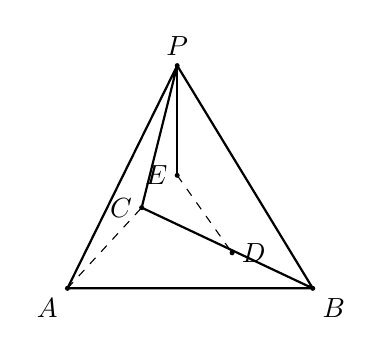
\begin{tikzpicture}[scale=0.82,>=stealth]
  \coordinate (P) at (1.7,3.45);
  \coordinate (A) at (0,0);
  \coordinate (B) at (3.8,0);
  \coordinate (C) at (1.15,1.25);
  \coordinate (E) at (1.7,1.75);
  \coordinate (D) at (2.55,0.55);
  \draw[thick] (P)--(A) (P)--(B) (P)--(C) (A)--(B) (B)--(C);
  \draw[dashed] (A)--(C) (E)--(D);
  \draw[thick] (E)--(P);
  \fill (P) circle (1.1pt) node[above] {$P$};
  \fill (A) circle (1.1pt) node[below left] {$A$};
  \fill (B) circle (1.1pt) node[below right] {$B$};
  \fill (C) circle (1.1pt) node[left] {$C$};
  \fill (E) circle (1.1pt) node[left] {$E$};
  \fill (D) circle (1.1pt) node[right] {$D$};
\end{tikzpicture}
\end{center}
\nopagebreak[4]
\Needspace{4\baselineskip}
\textbf{解析}

\Needspace{5\baselineskip}
取 $PA,BC,ED$ 为三个互相垂直的方向，并以 $A$ 为参考点。四面体体积为

\nopagebreak[4]
\[
V=\frac16\left|\det(\overrightarrow{AP},\overrightarrow{AB},\overrightarrow{AC})\right|.
\]

\Needspace{5\baselineskip}
因 $PA=BC=L$ 且 $PA\perp BC$，有

\nopagebreak[4]
\[
|\overrightarrow{AP}\times\overrightarrow{BC}|=L^2.
\]

\Needspace{5\baselineskip}
再乘以两条异面直线公垂线的距离 $ED=h$，混合积的绝对值为 $L^2h$，从而

\nopagebreak[4]
\[
V=\frac16L^2h.
\]

\gkanswer{答案：见解析正文。}

\end{answer}
\begin{answer}
\gksolhead{19}{}

\textbf{题目}：

\Needspace{5\baselineskip}
设对所有实数 $x$，不等式

\nopagebreak[4]
\[
x^2\log_2\frac{4(a+1)}a
+2x\log_2\frac{2a}{a+1}
+\log_2\frac{(a+1)^2}{4a^2}>0
\]

恒成立，求 $a$ 的取值范围。

\Needspace{4\baselineskip}
\textbf{解析}

\Needspace{5\baselineskip}
令

\nopagebreak[4]
\[
q=\log_2\frac{2a}{a+1}.
\]

\Needspace{5\baselineskip}
则

\nopagebreak[4]
\[
\log_2\frac{4(a+1)}a=3-q,\qquad
\log_2\frac{(a+1)^2}{4a^2}=-2q.
\]

\Needspace{5\baselineskip}
原式成为

\nopagebreak[4]
\[
(3-q)x^2+2qx-2q>0.
\]

\Needspace{5\baselineskip}
对一切实数 $x$ 恒正，必要条件由 $x=0$ 给出 $q<0$；此时二次项系数为正，判别式

\nopagebreak[4]
\[
\Delta=4q^2-4(3-q)(-2q)=4q(6-q)<0,
\]

\Needspace{5\baselineskip}
条件也充分。因此

\nopagebreak[4]
\[
0<\frac{2a}{a+1}<1.
\]

\Needspace{5\baselineskip}
结合对数定义域，得到

\nopagebreak[4]
\[
0<a<1.
\]

\gkanswer{答案：$0<a<1$}

\end{answer}
\begin{answer}
\gksolhead{20}{}

\textbf{题目}：

\Needspace{5\baselineskip}
设复数 $z_1$ 和 $z_2$ 满足关系式

\nopagebreak[4]
\[
z_1\overline{z_2}+\overline A z_1+A\overline{z_2}=0,
\]

其中 $A$ 为不等于 0 的复数。证明：

\Needspace{5\baselineskip}
（1） 证明：

\nopagebreak[4]
\[
|z_1+A||z_2+A|=|A|^2
\]
；

\Needspace{5\baselineskip}
（2） 证明：

\nopagebreak[4]
\[
\frac{z_1+A}{z_2+A}
=\left|
\frac{\overline{z_1}+\overline A}
{\overline{z_2}+\overline A}
\right|
\]
。

\Needspace{4\baselineskip}
\textbf{解析}

\gksubpart{（1）}

\Needspace{5\baselineskip}
由题设加上 $|A|^2=A\overline A$：

\nopagebreak[4]
\[
(z_1+A)(\overline{z_2}+\overline A)=|A|^2.
\]

\Needspace{5\baselineskip}
取绝对值得

\nopagebreak[4]
\[
|z_1+A||z_2+A|=|A|^2.
\]

\gksubpart{（2）}

\Needspace{5\baselineskip}
再除以 $|z_2+A|^2$，可得

\nopagebreak[4]
\[
\frac{z_1+A}{z_2+A}
=\frac{|A|^2}{|z_2+A|^2}
=\left|
\frac{\overline{z_1}+\overline A}
{\overline{z_2}+\overline A}
\right|.
\]

这同时给出题目的两个证明结论。

\gkanswer{答案（1）：见解析正文。}

\gkanswer{答案（2）：见解析正文。}

\end{answer}
\begin{answer}
\gksolhead{21}{}

\textbf{题目}：

\Needspace{5\baselineskip}
设数列 $a_1,a_2,\ldots,a_n,\ldots$ 的前 $n$ 项的和 $S_n$ 与 $a_n$ 满足

\nopagebreak[4]
\[
S_n=ka_n+1,
\]

其中 $k$ 是与 $n$ 无关的常数，且 $k\ne1$。

（1） 试写出用 $n,k$ 表示的 $a_n$ 的表达式；

\Needspace{5\baselineskip}
（2） 若

\nopagebreak[4]
\[
\lim_{n\to\infty}S_n=1,
\]

求 $k$ 的取值范围。

\Needspace{4\baselineskip}
\textbf{解析}

\gksubpart{（1）}

\Needspace{5\baselineskip}
由 $S_1=a_1=ka_1+1$ 得

\nopagebreak[4]
\[
a_1=\frac1{1-k}.
\]

\gksubpart{（2）}

\Needspace{5\baselineskip}
对 $n\ge2$，相减相邻两式：

\nopagebreak[4]
\[
a_n=S_n-S_{n-1}=k(a_n-a_{n-1}),
\]

\Needspace{5\baselineskip}
所以

\nopagebreak[4]
\[
a_n=\frac{k}{k-1}a_{n-1}.
\]

\Needspace{5\baselineskip}
故

\nopagebreak[4]
\[
a_n=\frac1{1-k}\left(\frac{k}{k-1}\right)^{n-1}
=\frac{(-k)^{n-1}}{(1-k)^n}.
\]

\Needspace{5\baselineskip}
并且

\nopagebreak[4]
\[
S_n=ka_n+1
=1-\left(\frac{k}{k-1}\right)^n.
\]

\Needspace{5\baselineskip}
要使 $S_n\to1$，须且只须

\nopagebreak[4]
\[
\left|\frac{k}{k-1}\right|<1,
\]

即 $k<\frac12$。

\gkanswer{答案（1）：$\displaystyle a_n=\frac{(-k)^{n-1}}{(1-k)^n}$}

\gkanswer{答案（2）：$k<\dfrac12$}

\end{answer}
\begin{answer}
\gksolhead{22}{}

\textbf{题目}：

\Needspace{5\baselineskip}
正方形 $ABCD$ 在直角坐标平面内，已知其一条边 $AB$ 在直线

\nopagebreak[4]
\[
y=x+4
\]

\Needspace{5\baselineskip}
上，$C,D$ 在抛物线

\nopagebreak[4]
\[
x=y^2
\]

上，求正方形 $ABCD$ 的面积。

\Needspace{4\baselineskip}
\textbf{解析}

\Needspace{5\baselineskip}
设抛物线上的两个顶点为

\nopagebreak[4]
\[
C=(u^2,u),\qquad D=(v^2,v).
\]

\Needspace{5\baselineskip}
因 $AB\parallel CD$ 且 $AB$ 的斜率为 1，有

\nopagebreak[4]
\[
u^2-v^2=u-v.
\]

\Needspace{5\baselineskip}
两点不重合，故 $u+v=1$。令 $t=u-v$，则正方形边长为 $\sqrt2|t|$。另一方面，两条平行边 $AB$ 与 $CD$ 的距离为

\nopagebreak[4]
\[
\frac{|v^2-v+4|}{\sqrt2}.
\]

\Needspace{5\baselineskip}
令两者相等，得

\nopagebreak[4]
\[
v^2-v+4=2|1-2v|.
\]

\Needspace{5\baselineskip}
分两种情况：

\nopagebreak[4]
\[
v\le\frac12\Longrightarrow(v+1)(v+2)=0,
\]

\nopagebreak[4]
\[
v\ge\frac12\Longrightarrow(v-2)(v-3)=0.
\]

\Needspace{5\baselineskip}
于是 $|1-2v|$ 为 $3$ 或 $5$，正方形面积分别为

\nopagebreak[4]
\[
(\sqrt2\cdot3)^2=18,\qquad
(\sqrt2\cdot5)^2=50.
\]

\Needspace{5\baselineskip}
两个值均可实现，例如相应顶点可取

\nopagebreak[4]
\[
(-2,2),(1,5),(4,2),(1,-1)
\]

\Needspace{5\baselineskip}
或

\nopagebreak[4]
\[
(-1,3),(4,8),(9,3),(4,-2).
\]

因此按固定源题面，所求面积为 $18$ 或 $50$；若原题另有未见的选项/位置限制，需要独立源才能裁决。

\gkanswer{答案：$18$ 或 $50$}

\end{answer}